%%%%%%%%%%%%%%%%%%%%%%%%%%%%%%%%%%%%%%%%%%%%%%%%%%%%%%%%%%%%%%%
%% OXFORD THESIS TEMPLATE

% Use this template to produce a standard thesis that meets the Oxford University requirements for DPhil submission
%
% Originally by Keith A. Gillow (gillow@maths.ox.ac.uk), 1997
% Modified by Sam Evans (sam@samuelevansresearch.org), 2007
% Modified by John McManigle (john@oxfordechoes.com), 2015
%
% This version Copyright (c) 2015-2017 John McManigle
%
% Broad permissions are granted to use, modify, and distribute this software
% as specified in the MIT License included in this distribution's LICENSE file.
%

% I've (John) tried to comment this file extensively, so read through it to see how to use the various options.  Remember
% that in LaTeX, any line starting with a % is NOT executed.  Several places below, you have a choice of which line to use
% out of multiple options (eg draft vs final, for PDF vs for binding, etc.)  When you pick one, add a % to the beginning of
% the lines you don't want.


%%%%% CHOOSE PAGE LAYOUT
% The most common choices should be below.  You can also do other things, like replacing "a4paper" with "letterpaper", etc.

% This one will format for two-sided binding (ie left and right pages have mirror margins; blank pages inserted where needed):
\documentclass[a4paper,twoside]{ociamthesis}
% This one will format for one-sided binding (ie left margin > right margin; no extra blank pages):
%\documentclass[a4paper]{ociamthesis}
% This one will format for PDF output (ie equal margins, no extra blank pages):
%\documentclass[a4paper,nobind]{ociamthesis} 

\newcommand\ion[2]{#1$\;${\scshape{#2}}}%                       % ion, i.e., CII = \ion{C}{ii}
\newcommand{\kms}{km\,s$^{-1}$}
\newcommand{\SN}{S$/$N}
\newcommand{\hi}{\ion{H}{i}}
\newcommand{\hii}{\ion{H}{ii}}
\newcommand{\hei}{\ion{He}{i}}
\newcommand{\heii}{\ion{He}{ii}}
\newcommand{\Ni}{[\ion{N}{i}]}
\newcommand{\nii}{[\ion{N}{ii}]}
\newcommand{\oi}{[\ion{O}{i}]}
\newcommand{\OI}{\ion{O}{i}}
\newcommand{\oii}{[\ion{O}{ii}]}
\newcommand{\oiii}{[\ion{O}{iii}]}
\newcommand{\sii}{[\ion{S}{ii}]}
\newcommand{\siii}{[\ion{S}{iii}]}
\newcommand{\ha}{H$\alpha$} 
\newcommand{\hb}{H$\beta$} 
\newcommand{\feii}{[\ion{Fe}{ii}]}
\newcommand{\cliii}{[\ion{Cl}{iii}]}
\newcommand{\ariii}{[\ion{Ar}{iii}]}
\newcommand{\SiII}{\ion{Si}{ii}}

\newcommand{\flux}{erg\,s$^{-1}$\,cm$^{-2}$}
%\newcommand{\HII}{\ion{H}{2}}
%\newcommand{\Com}[1]{{\color{red}*** #1}}
\newcommand{\temp}{T$_{\rm e}$}
\newcommand{\EWha}{W$_{{\rm H}\alpha}$}



\newcommand{\apj}{ApJ}
\newcommand{\apjl}{ApJ}
\newcommand{\mnras}{MNRAS}
\newcommand{\aap}{A\&A}
\newcommand{\aj}{AJ}
\newcommand{\nat}{Nature}
\newcommand{\pre}{Phys.~Rev.~E}
\newcommand{\araa}{ARA\&A}
\newcommand{\rmxaa}{RMxAA}
\newcommand{\icarus}{Icarus}


%%%%% SELECT YOUR DRAFT OPTIONS
% Three options going on here; use in any combination.  But remember to turn the first two off before
% generating a PDF to send to the printer!

% This adds a "DRAFT" footer to every normal page.  (The first page of each chapter is not a "normal" page.)
\fancyfoot[C]{\emph{DRAFT Printed on \today}}  

% This highlights (in blue) corrections marked with (for words) \mccorrect{blah} or (for whole
% paragraphs) \begin{mccorrection} . . . \end{mccorrection}.  This can be useful for sending a PDF of
% your corrected thesis to your examiners for review.  Turn it off, and the blue disappears.
\correctionstrue


%%%%% BIBLIOGRAPHY SETUP
% Note that your bibliography will require some tweaking depending on your department, preferred format, etc.
% The options included below are just very basic "sciencey" and "humanitiesey" options to get started.
% If you've not used LaTeX before, I recommend reading a little about biblatex/biber and getting started with it.
% If you're already a LaTeX pro and are used to natbib or something, modify as necessary.
% Either way, you'll have to choose and configure an appropriate bibliography format...

% The science-type option: numerical in-text citation with references in order of appearance.
\usepackage[style=numeric-comp, sorting=none, backend=biber, doi=false, isbn=false]{biblatex}
\newcommand*{\bibtitle}{References}

% The humanities-type option: author-year in-text citation with an alphabetical works cited.
%\usepackage[style=authoryear, sorting=nyt, backend=biber, maxcitenames=2, useprefix, doi=false, isbn=false]{biblatex}
%\newcommand*{\bibtitle}{Works Cited}

% This makes the bibliography left-aligned (not 'justified') and slightly smaller font.
\renewcommand*{\bibfont}{\raggedright\small}

% Change this to the name of your .bib file (usually exported from a citation manager like Zotero or EndNote).
\addbibresource{tesis.bib}


% Uncomment this if you want equation numbers per section (2.3.12), instead of per chapter (2.18):
%\numberwithin{equation}{subsection}



%%%%% THESIS / TITLE PAGE INFORMATION
% Everybody needs to complete the following:
\title{Systematic study of outflows in the Local Universe}
\author{Carlos L\'opez Cob\'a}
\college{Instituto de Astronom\'ia}

% Master's candidates who require the alternate title page (with candidate number and word count)
% must also un-comment and complete the following three lines:
%\masterssubmissiontrue
%\candidateno{933516}
%\wordcount{28,815}

% Uncomment the following line if your degree also includes exams (eg most masters):
%\renewcommand{\submittedtext}{Submitted in partial completion of the}
% Your full degree name.  (But remember that DPhils aren't "in" anything.  They're just DPhils.)
\degree{Doctor of Philosophy}
% Term and year of submission, or date if your board requires (eg most masters)
\degreedate{Michaelmas 2014}


%%%%% YOUR OWN PERSONAL MACROS
% This is a good place to dump your own LaTeX macros as they come up.

% To make text superscripts shortcuts
	\renewcommand{\th}{\textsuperscript{th}} % ex: I won 4\th place
	\newcommand{\nd}{\textsuperscript{nd}}
	\renewcommand{\st}{\textsuperscript{st}}
	\newcommand{\rd}{\textsuperscript{rd}}

%%%%% THE ACTUAL DOCUMENT STARTS HERE
\begin{document}



%%%%% CHOOSE YOUR LINE SPACING HERE
% This is the official option.  Use it for your submission copy and library copy:
\setlength{\textbaselineskip}{22pt plus2pt}
% This is closer spacing (about 1.5-spaced) that you might prefer for your personal copies:
%\setlength{\textbaselineskip}{18pt plus2pt minus1pt}

% You can set the spacing here for the roman-numbered pages (acknowledgements, table of contents, etc.)
\setlength{\frontmatterbaselineskip}{17pt plus1pt minus1pt}

% Leave this line alone; it gets things started for the real document.
\setlength{\baselineskip}{\textbaselineskip}


%%%%% CHOOSE YOUR SECTION NUMBERING DEPTH HERE
% You have two choices.  First, how far down are sections numbered?  (Below that, they're named but
% don't get numbers.)  Second, what level of section appears in the table of contents?  These don't have
% to match: you can have numbered sections that don't show up in the ToC, or unnumbered sections that
% do.  Throughout, 0 = chapter; 1 = section; 2 = subsection; 3 = subsubsection, 4 = paragraph...

% The level that gets a number:
\setcounter{secnumdepth}{2}
% The level that shows up in the ToC:
\setcounter{tocdepth}{2}


%%%%% ABSTRACT SEPARATE
% This is used to create the separate, one-page abstract that you are required to hand into the Exam
% Schools.  You can comment it out to generate a PDF for printing or whatnot.
\begin{abstractseparate}
	Your abstract text goes here.  Check your departmental regulations, but generally this should be less than 300 words.  See the beginning of Chapter~\ref{ch:2-litreview} for more.

Lorem ipsum dolor sit amet, consectetur adipiscing elit. Pellentesque sit amet nibh volutpat, scelerisque nibh a, vehicula neque. Integer placerat nulla massa, et vestibulum velit dignissim id. Ut eget nisi elementum, consectetur nibh in, condimentum velit. Quisque sodales dui ut tempus mattis. Duis malesuada arcu at ligula egestas egestas. Phasellus interdum odio at sapien fringilla scelerisque. Mauris sagittis eleifend sapien, sit amet laoreet felis mollis quis. Pellentesque dui ante, finibus eget blandit sit amet, tincidunt eu neque. Vivamus rutrum dapibus ligula, ut imperdiet lectus tincidunt ac. Pellentesque ac lorem sed diam egestas lobortis.

Suspendisse leo purus, efficitur mattis urna a, maximus molestie nisl. Aenean porta semper tortor a vestibulum. Suspendisse viverra facilisis lorem, non pretium erat lacinia a. Vestibulum tempus, quam vitae placerat porta, magna risus euismod purus, in viverra lorem dui at metus. Sed ac sollicitudin nunc. In maximus ipsum nunc, placerat maximus tortor gravida varius. Suspendisse pretium, lorem at porttitor rhoncus, nulla urna condimentum tortor, sed suscipit nisi metus ac risus.

Aenean sit amet enim quis lorem tristique commodo vitae ut lorem. Duis vel tincidunt lacus. Sed massa velit, lacinia sed posuere vitae, malesuada vel ante. Praesent a rhoncus leo. Etiam sed rutrum enim. Pellentesque lobortis elementum augue, at suscipit justo malesuada at. Lorem ipsum dolor sit amet, consectetur adipiscing elit. Praesent rhoncus convallis ex. Etiam commodo nunc ex, non consequat diam consectetur ut. Pellentesque vitae est nec enim interdum dapibus. Donec dapibus purus ipsum, eget tincidunt ex gravida eget. Donec luctus nisi eu fringilla mollis. Donec eget lobortis diam.

Suspendisse finibus placerat dolor. Etiam ornare elementum ex ut vehicula. Donec accumsan mattis erat. Quisque cursus fringilla diam, eget placerat neque bibendum eu. Ut faucibus dui vitae dolor porta, at elementum ipsum semper. Sed ultrices dui non arcu pellentesque placerat. Etiam posuere malesuada turpis, nec malesuada tellus malesuada. % Create an abstract.tex file in the 'text' folder for your abstract.
\end{abstractseparate}


% JEM: Pages are roman numbered from here, though page numbers are invisible until ToC.  This is in
% keeping with most typesetting conventions.
\begin{romanpages}

% Title page is created here
\maketitle

%%%%% DEDICATION -- If you'd like one, un-comment the following.
%\begin{dedication}
%This thesis is dedicated to\\
%someone\\
%for some special reason\\
%\end{dedication}

%%%%% ACKNOWLEDGEMENTS -- Nothing to do here except comment out if you don't want it.
\begin{acknowledgements}
Aqui los agradecimientos
 	%\subsection*{Personal}

This is where you thank your advisor, colleagues, and family and friends.

Lorem ipsum dolor sit amet, consectetur adipiscing elit. Vestibulum feugiat et est at accumsan. Praesent sed elit mattis, congue mi sed, porta ipsum. In non ullamcorper lacus. Quisque volutpat tempus ligula ac ultricies. Nam sed erat feugiat, elementum dolor sed, elementum neque. Aliquam eu iaculis est, a sollicitudin augue. Cras id lorem vel purus posuere tempor. Proin tincidunt, sapien non dictum aliquam, ex odio ornare mauris, ultrices viverra nisi magna in lacus. Fusce aliquet molestie massa, ut fringilla purus rutrum consectetur. Nam non nunc tincidunt, rutrum dui sit amet, ornare nunc. Donec cursus tortor vel odio molestie dignissim. Vivamus id mi erat. Duis porttitor diam tempor rutrum porttitor. Lorem ipsum dolor sit amet, consectetur adipiscing elit. Sed condimentum venenatis consectetur. Lorem ipsum dolor sit amet, consectetur adipiscing elit.

Aenean sit amet lectus nec tellus viverra ultrices vitae commodo nunc. Mauris at maximus arcu. Aliquam varius congue orci et ultrices. In non ipsum vel est scelerisque efficitur in at augue. Nullam rhoncus orci velit. Duis ultricies accumsan feugiat. Etiam consectetur ornare velit et eleifend.

Suspendisse sed enim lacinia, pharetra neque ac, ultricies urna. Phasellus sit amet cursus purus. Quisque non odio libero. Etiam iaculis odio a ex volutpat, eget pulvinar augue mollis. Mauris nibh lorem, mollis quis semper quis, consequat nec metus. Etiam dolor mi, cursus a ipsum aliquam, eleifend venenatis ipsum. Maecenas tempus, nibh eget scelerisque feugiat, leo nibh lobortis diam, id laoreet purus dolor eu mauris. Pellentesque habitant morbi tristique senectus et netus et malesuada fames ac turpis egestas. Nulla eget tortor eu arcu sagittis euismod fermentum id neque. In sit amet justo ligula. Donec rutrum ex a aliquet egestas.

\subsection*{Institutional}

If you want to separate out your thanks for funding and institutional support, I don't think there's any rule against it.  Of course, you could also just remove the subsections and do one big traditional acknowledgement section.

Lorem ipsum dolor sit amet, consectetur adipiscing elit. Ut luctus tempor ex at pretium. Sed varius, mauris at dapibus lobortis, elit purus tempor neque, facilisis sollicitudin felis nunc a urna. Morbi mattis ante non augue blandit pulvinar. Quisque nec euismod mauris. Nulla et tellus eu nibh auctor malesuada quis imperdiet quam. Sed eget tincidunt velit. Cras molestie sem ipsum, at faucibus quam mattis vel. Quisque vel placerat orci, id tempor urna. Vivamus mollis, neque in aliquam consequat, dui sem volutpat lorem, sit amet tempor ipsum felis eget ante. Integer lacinia nulla vitae felis vulputate, at tincidunt ligula maximus. Aenean venenatis dolor ante, euismod ultrices nibh mollis ac. Ut malesuada aliquam urna, ac interdum magna malesuada posuere.
\end{acknowledgements}

%%%%% ABSTRACT -- Nothing to do here except comment out if you don't want it.
\begin{abstract}
The present thesis abords the detection and characterization of galactic scale outflows trough the use of 
integral field spectroscopy technique.

%Your abstract text goes here.  Check your departmental regulations, but generally this should be less than 300 words.  See the beginning of Chapter~\ref{ch:2-litreview} for more.

Lorem ipsum dolor sit amet, consectetur adipiscing elit. Pellentesque sit amet nibh volutpat, scelerisque nibh a, vehicula neque. Integer placerat nulla massa, et vestibulum velit dignissim id. Ut eget nisi elementum, consectetur nibh in, condimentum velit. Quisque sodales dui ut tempus mattis. Duis malesuada arcu at ligula egestas egestas. Phasellus interdum odio at sapien fringilla scelerisque. Mauris sagittis eleifend sapien, sit amet laoreet felis mollis quis. Pellentesque dui ante, finibus eget blandit sit amet, tincidunt eu neque. Vivamus rutrum dapibus ligula, ut imperdiet lectus tincidunt ac. Pellentesque ac lorem sed diam egestas lobortis.

Suspendisse leo purus, efficitur mattis urna a, maximus molestie nisl. Aenean porta semper tortor a vestibulum. Suspendisse viverra facilisis lorem, non pretium erat lacinia a. Vestibulum tempus, quam vitae placerat porta, magna risus euismod purus, in viverra lorem dui at metus. Sed ac sollicitudin nunc. In maximus ipsum nunc, placerat maximus tortor gravida varius. Suspendisse pretium, lorem at porttitor rhoncus, nulla urna condimentum tortor, sed suscipit nisi metus ac risus.

Aenean sit amet enim quis lorem tristique commodo vitae ut lorem. Duis vel tincidunt lacus. Sed massa velit, lacinia sed posuere vitae, malesuada vel ante. Praesent a rhoncus leo. Etiam sed rutrum enim. Pellentesque lobortis elementum augue, at suscipit justo malesuada at. Lorem ipsum dolor sit amet, consectetur adipiscing elit. Praesent rhoncus convallis ex. Etiam commodo nunc ex, non consequat diam consectetur ut. Pellentesque vitae est nec enim interdum dapibus. Donec dapibus purus ipsum, eget tincidunt ex gravida eget. Donec luctus nisi eu fringilla mollis. Donec eget lobortis diam.

Suspendisse finibus placerat dolor. Etiam ornare elementum ex ut vehicula. Donec accumsan mattis erat. Quisque cursus fringilla diam, eget placerat neque bibendum eu. Ut faucibus dui vitae dolor porta, at elementum ipsum semper. Sed ultrices dui non arcu pellentesque placerat. Etiam posuere malesuada turpis, nec malesuada tellus malesuada.
\end{abstract}

%%%%% MINI TABLES
% This lays the groundwork for per-chapter, mini tables of contents.  Comment the following line
% (and remove \minitoc from the chapter files) if you don't want this.  Un-comment either of the
% next two lines if you want a per-chapter list of figures or tables.
\dominitoc % include a mini table of contents
%\dominilof  % include a mini list of figures
%\dominilot  % include a mini list of tables

% This aligns the bottom of the text of each page.  It generally makes things look better.
\flushbottom

% This is where the whole-document ToC appears:
\tableofcontents

\listoffigures
	\mtcaddchapter
% \mtcaddchapter is needed when adding a non-chapter (but chapter-like) entity to avoid confusing minitoc

% Uncomment to generate a list of tables:
%\listoftables
%	\mtcaddchapter

%%%%% LIST OF ABBREVIATIONS
% This example includes a list of abbreviations.  Look at text/abbreviations.tex to see how that file is
% formatted.  The template can handle any kind of list though, so this might be a good place for a
% glossary, etc.
% First parameter can be changed eg to "Glossary" or something.
% Second parameter is the max length of bold terms.
\begin{mclistof}{List of Abbreviations}{3.2cm}

\item[AGN] Active galactic nuclei.

\item[CALIFA] Calar Alto Legacy Integral Field Area Survey.

\item[FoV] Field-of-View. 

\item[IFS] Integral field spectroscopy.

\item[IFU] Integral field unit.

\item[IMF] Initial mass function.

\item[MaNGA] Mapping Nearby Galaxies at APO.

\item[MUSE] Multi Unit Spectroscopic Explorer. 

\item[NIR] Near Infra Red.

\item[R$_e$] Effective radius.

\item[SAMI] Sydney-AAO Multi-object Integral field spectrograph.

\item[SF] Star formation.

\item[SFR] Star formation rate.

\item[SFMS] Star formation main sequence.

\item[SMBH] Super massive black hole.

\item[SNe] Supernovae.

\item[QSO] Quasi-stellar object.

\item[SSP] Simple stellar popularion.

\item[UV] Ultraviolet.





\end{mclistof} 


% The Roman pages, like the Roman Empire, must come to its inevitable close.
\end{romanpages}


%%%%% CHAPTERS
% Add or remove any chapters you'd like here, by file name (excluding '.tex'):
\flushbottom
\begin{savequote}[8cm]
\textlatin{Neque porro quisquam est qui dolorem ipsum quia dolor sit amet, consectetur, adipisci velit...}

There is no one who loves pain itself, who seeks after it and wants to have it, simply because it is pain...
  \qauthor{--- Cicero's \textit{de Finibus Bonorum et Malorum}}
\end{savequote}

\chapter{\label{ch:1-intro}Introduction} 

\minitoc

\section{Motivation}

Intense star formation in galaxies as well as active galactic nuclei can drive the ejection of gas in different phaces (neutral, ionized, molecular) out of a galaxy.
The ejected gas, can reach up to hundreds to kiloparsec scales, becoming large--scale galactic outflows drived by SF-process, AGN activity or both.

Despite its plenity identification at low and high redshift (tipically constrained its detection between $0<z<2$), its main physical mechanism(s) that produces
and regulates its production is(are) still unclear. The most common mechanism to detect them is trough emission and absorption lines (molecular, optical, UV, NIR, soft Xray). 

The wind leaves signatues in the spectrum as broad or assimetric profiles, indicative of the precense of distint kinematic components as result of the propagion of the wind.
As more intense the wind energy source, higher the velocity. Therefore, a disturbed kinematic in the galaxy velocity field, is a condition to reveal the precense of an outflow (both AGN or SF driven), 
although this is not definitive. 
 
Given the large amount of energy  realezed ($\sim 10^{xx}$ erg s-1), and posterior inject back to the host galaxy, its
consequences might change the subsequent evolution of the host galaxy itself. 

The main energy sources that produce galactic scale outflows are: (i) Supernovae (SNe) explosions. Intense star formation rates as those present in starburst galaxies are prone to
develop large scale outflows. At the end of its life, massive stars (10 M$_{\odot}$) end up as SNe, the relative short live of these stars and its inmediate explosion as SNe
delivers amounts of energy to the ISM. The joint effect of multiple SN explosions drives as a expanding shell is now well uderstood (Heckman 1990). From this, it is not surprising that
the total energy of SNs is directly related with the globlal SFR of a galaxy. 


(ii) Nuclear activity. The accretion of material into super massive black holes (SMBH) in the center of galaxies can lead to the production of higly energetic outflows (AGN-driven), tipically preceded
by a radio jet. The more luminous the AGN is, major its velocity, reaching in the most luminous cases up to $~10^3$ \kms. 

Commonly the study of outflows has been performed over galaxy samples where its precesen is ubiquitous. This is, in galaxies with high star formation rates, in the 
so called ultra luminous infrared galaxies (ULIRGs), or in the most luminous AGNs, such as QSO. Although all these studies has contributed to expand our knoledge to the outflows phenomena.

All these studies have consolidated our current knowledge about the outflows, where to find them and how estimate its main physical properties,as well as the
limitations. Nowadays with the advent of large galaxy surveys it is possible to perform unbiased studies. One of the major questions that attend to answer in this thesis is
on how frequent they are, and why they seem to be  not ubiquitous in all galaxies. 
 

\section{Integral Field Spectroscopy}
In the late 90s and early 2000s, a new observation technique came to light to overcome the classical long slit spectroscopy. The
integral field spectroscopy (IFS) technique produces simultaneously multiple spatially resolved spectra over a two dimensional field \cite{bookIFS}. This technique
bringing back the study of extended objects, instead the one sigle fiber, or long slit spectroscopy. The IFS technique
provides a 3 dimensional vission of a galaxy, two dimensions $(x,y)$ corresponds to the spatiall  information (R.A.,Dec), and the $z$ axis corresponds to the wavelength axis.
How the information is recorded depends on the type of integral field unit (IFU). The most common are represented in Fig. \ref{fig:ifs}. 
The final reduction process results in a data cube, where each of its spatial elements (spaxels) records the spectroscopic information of a small portion of a galaxy. The gread advantage of this
technique is the possibility of study the individual structural components of galaxyes (such as bars, disk, bulge, spiral arms, \hii~regions etc.)

The large programs to study galaxies using the IFS technique started with the SAURON project \cite{bacon01}. SAURON was optimized to study the stellar kinematics of nearby early-type galaxies.
Followed SAURON, the SAMI Galaxy Survey \cite{samiOLD} came to light with more than $\sim 3400$ low redshift galaxies ($z<0.12$). 

The larger program in observed galaxies is the MaNGA survey \cite{mangaOLD}, aiming to observe $\sim 10000$ galaxies from the Local Universe. The CALIFA survey \cite{sanchez12a} is the last IFS galaxy
survey delivering $~800$ galaxies of the Local Universe. 

Many MUSE IFS projects has been proposed to study with high spatial resoluion the physical properties of low and high redshift galaxies. Although there is not yet a proper MUSE galaxy survey,
the AMUSING++ compilation has collected the major number of galaxies observed with MUSE so far. 

Table \ref{tab:IFS_properties} sumarizes the main properties of the main IFS galaxy surveys.

\begin{sidewaystable} 
\begin{tabular}{lllrlll}
\toprule
 Survey    & redshift      & R         &   N\_gal & FWHM (arcsec)   & FoV (arcsec)   & lambda\_range (Angs)   \\
\midrule
 SAMI      & 0.004\ensuremath{<}z\ensuremath{<}0.092 & 1700,4500 &    1559 & 2.16            & 15x15          & 3700--7300            \\
 MaNGA     & 0.025\ensuremath{<}z\ensuremath{<}0.15  & 1400-2600 &   10000 & 2.54,2.48       & 7-32           & 4000--9000            \\
 CALIFA    & 0.005\ensuremath{<}z\ensuremath{<}0.03  & 850,1650  &     667 & 2.5             & 78x73          & 3745--7500            \\
 AMUSING++ & 0.001\ensuremath{<}z\ensuremath{<}0.1   & 3000      &     700 & seeing limited  & 60x60          & 4800--9300            \\
\bottomrule
\end{tabular}
\label{tab:IFS_properties}
\caption{Main IFS galaxy surveys}
\end{sidewaystable} 


\begin{figure}
\centering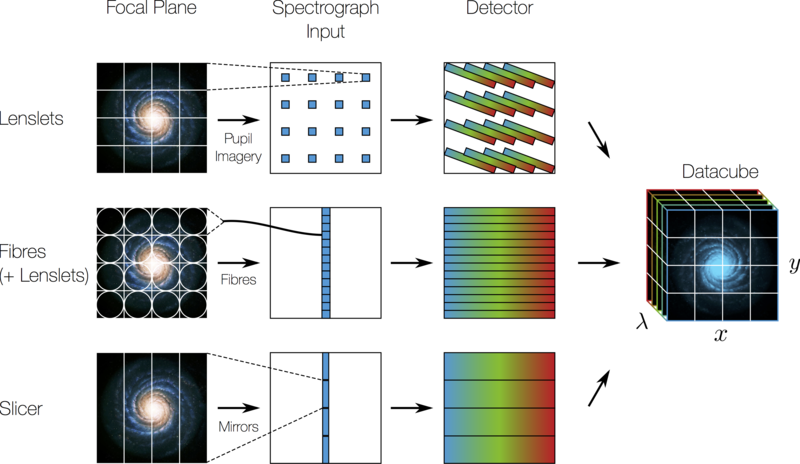
\includegraphics[width=0.7\textwidth]{figures/ifs.png} 
\caption[]{Diffeerent types of IFU. }
\label{fig:ifs}
\end{figure}


\section{Data}
The current work is based on data from extracted from the CALIFA survey \url{https://califa.caha.es} and MUSE data \url{http://ifs.astroscu.unam.mx/AMUSING++}.

\subsection{CALIFA}
The CALIFA project has been one of the most successful IFS galaxy surveys, mostly because of its well-designed sample.
CALIFA is a diameter selection sample, covering up to 2 effective radius (R$_e$) in the vast majority of the galaxies. 
The diameter selection condition allowed to perform volume corrections over the sample within
the redshift range of the galaxies. This great adventage has allowed to estimate statistical properties of the sample, and therefore of the Local Universe. 

The vast coverage of the blue and red part of the optical spectrum allows recovering the information of the stellar component trough the appropriate SSP fitting analysis techniques. Moreover, the most prominent emission lines in the optical spectrum are totally sampled.

Given its large FoV, the CALIFA galaxies can be studied spatially resolved (spaxel-by-spaxel), globally (integrated) or radially. Therefore, the way in which galaxies are studied 
has changed dramatically with the adevent of the most modern IFS techiques, particulary with the CALIFA survey has opened a branche towards the 3 dimensional study of galaxies.

\subsection{MUSE}

Installed at the  Very Large Telescope in the southern hemisphere, the Multi Unit Spectroscopic Explorer (MUSE) is the most modern instrument for obtaining IFS data in the optical. MUSE
provides a high spatial resolution limited by the local seeing, and a moderated spectral resolution that depends on the wavelength. For the lowest redshift galaxies, MUSE can 
achive spatial resolutions of the order of $\sim 100$ pc (cite TIMER,MAD), pushing to the limit the established global scaling relations of galaxies, 
at unprecedent resolutions. 

Many extragalactic projects has been proposed to study the physical properties of galaxies at different scales.

The major disadvanatge of the current MUSE, is the lack of the blue part of the spectrum. 
Important absorptions lines in the blue part of the spectrum can help to break the well known age-metallicity degeneracy. 
A direct consequence of this degeneracy is the unreliability in the SSP analysis on the MUSE data cubes. 
Nevertheless, this degeneray do not affect the extraction of ionized gas properties.

Keeping in mind this caveat, many extragalactic projects has been proposed to study the physical
properties (particularly on the ionized gas) of galaxies at different scales. 

In this thesis, data from the public ESO archive has been used, in combination with data from other major MUSE programs, as it will be described in further sections.

%In general older stellar populations are redder, like metal rich ones, while younger and metal poor ones are bluer (Worthey 1994). This in troduces a degeneracy in the derivation of both parameters, as discussed by previous authors

\section{Data Analysis}

The spectra observed in a region of galaxy is the result of the contribution of all ionizing and continuum sources in that region. Particularly, at the redshift range of the
previous IFS galaxy surveys, the initial mass function (IMF) is not sampled at any of the previously cited spatial resolutions. Therefore, it is assumed that
in each spatiall element in a galaxy, the observed continuum spectrum is the combination of the sum of some thousands of stars, giving the shape of the continuum spectra in each spaxel.  

In order to recover the ionized and stellar content of galaxies, we perform a simple stellar population analys (SSP) analysis to each spectra of the datacubes.
To achive this, we use the {\sc Pipe3d} \cite{Pipe3D_I}, a fitting routine adapted to analyse IFS  data using the package {\sc FIT3d} \cite{Pipe3D_II}. A wide description
of how {\sc Pipe3d} works is described in  \cite{Pipe3D_I}. In general terms, this routine performs a decomposition of the original spectrum into SSP, 
prior to a coadding of adjacent spectra process in order to increase the \SN~of the continuum. This results in a segmented map of the galaxy in question. 
Over each segmented bin, also known as tessela, a SSP fitting is perfomed over the coaddes spectra. 
SSP templates of different ages and metallicities are used to perform this analysis. The fit is then monitored with a chi-squared minimization process. 
The final SSP model, contains information of the mean age, stellar mass and stellar metallicities. This is choosen as representative SSP model of the tessela. After that
an dezonification process is performed, to recover the . An example of this fitting procedure is sumarized in Fig. \ref{fig:ssp_fitting}. 

Once obtained the best SSP model, this is subtracted to the original spectra to obtain a spectrum free of stellar-continuum, this is, a gas
spectra dominated by pure emission lines (plus some residual noise). After this, the emission lines are fitted trough a moment analysis procedure to recover the flux, 
velocity and velocity dispersion with its corresponding errors for each analized emission line.

The previous proccedure applied to a entire datacube, produces a set of 2D maps of the stellar and ionized components. {\sc Pipe3d} packs the results of 
the analysis in datacubes, separated in the stellar and ionized gas information. These products are named dataproducts. 


\begin{figure*}
\centering
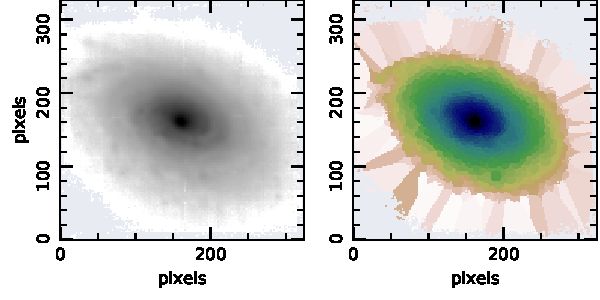
\includegraphics[width= \textwidth]{figures/tessela.pdf} 
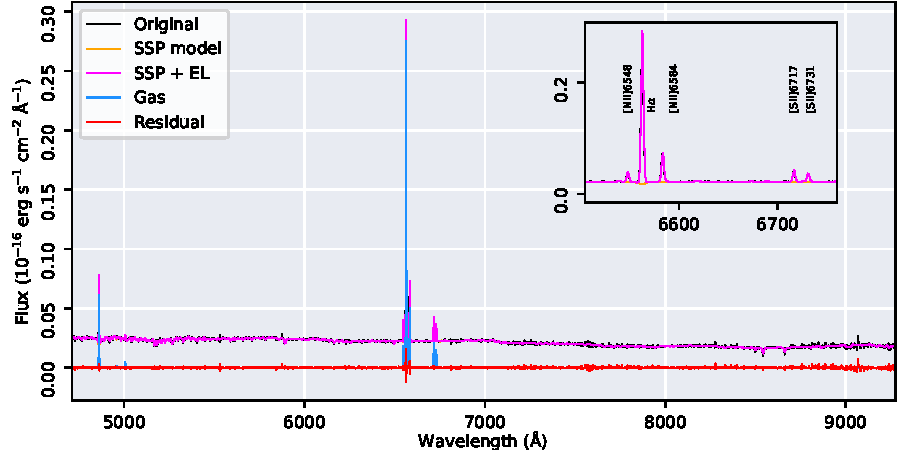
\includegraphics[width= \textwidth]{figures/ssp_fit_muse.pdf} 
\caption[]{Example of the SSP analysis applied to an IFS cube. In this example only a single spectrum of a tessela is analyzed. 
{\it Top left:} V--band continuum image extracted from the datacube. {\it Top right:} Tesselation map. 
{\it Bottom panel:} The {\sc Pipe3d} routine models the obseved spectra (black) with a combination of different SSP, the best model (orange) is
considered as the best   }
\label{fig:ssp_fitting}
\end{figure*}











\begin{savequote}[8cm]
Alles Gescheite ist schon gedacht worden.\\
Man muss nur versuchen, es noch einmal zu denken.

All intelligent thoughts have already been thought;\\
what is necessary is only to try to think them again.
  \qauthor{--- Johann Wolfgang von Goethe \cite{von_goethe_wilhelm_1829}}
\end{savequote}

\chapter{\label{ch:2-litreview}Background}

\minitoc

\section{The optical approch to the study of outflows}
As mentioned previously outflows are multiwavelength phenomena, capturing a different snapshot of the same phenomena in
different spectral bands.


\section{IFS and outflows}




%% APPENDICES %% 
% Starts lettered appendices, adds a heading in table of contents, and adds a
%    page that just says "Appendices" to signal the end of your main text.
\startappendices
% Add or remove any appendices you'd like here:
\begin{savequote}[8cm]
\textlatin{Cor animalium, fundamentum e\longs t vitæ, princeps omnium, Microco\longs mi Sol, a quo omnis vegetatio dependet, vigor omnis \& robur emanat.}

The heart of animals is the foundation of their life, the sovereign of everything within them, the sun of their microcosm, that upon which all growth depends, from which all power proceeds.
  \qauthor{--- William Harvey \cite{harvey_exercitatio_1628}}
\end{savequote}

\chapter{\label{app:1-cardiophys}Review of Cardiac Physiology and Electrophysiology}

\minitoc

Appendices are just like chapters.  Their sections and subsections get numbered and included in the table of contents; figures and equations and tables added up, etc.  Lorem ipsum dolor sit amet, consectetur adipiscing elit. Sed et dui sem. Aliquam dictum et ante ut semper. Donec sollicitudin sed quam at aliquet. Sed maximus diam elementum justo auctor, eget volutpat elit eleifend. Curabitur hendrerit ligula in erat feugiat, at rutrum risus suscipit. Pellentesque habitant morbi tristique senectus et netus et malesuada fames ac turpis egestas. Integer risus nulla, facilisis eget lacinia a, pretium mattis metus. Vestibulum aliquam varius ligula nec consectetur. Maecenas ac ipsum odio. Cras ac elit consequat, eleifend ipsum sodales, euismod nunc. Nam vitae tempor enim, sit amet eleifend nisi. Etiam at erat vel neque consequat.

\section{Anatomy}
\label{sec:anatomy}

Lorem ipsum dolor sit amet, consectetur adipiscing elit. Donec accumsan cursus neque. Pellentesque eget tempor turpis, quis malesuada dui. Proin egestas, sapien sit amet feugiat vulputate, nunc nibh mollis nunc, nec auctor turpis purus sed metus. Aenean consequat leo congue volutpat euismod. Vestibulum et vulputate nisl, at ultrices ligula. Cras pulvinar lacinia ipsum at bibendum. In ac augue ut ante mollis molestie in a arcu.

Etiam vitae quam sollicitudin, luctus tortor eu, efficitur nunc. Vestibulum maximus, ante quis consequat sagittis, augue velit luctus odio, in scelerisque arcu magna id diam. Proin et mauris congue magna auctor pretium id sit amet felis. Maecenas sit amet lorem ipsum. Proin a risus diam. Integer tempus eget est condimentum faucibus. Suspendisse sem metus, consequat vel ante eget, porttitor maximus dui. Nunc dapibus tincidunt enim, non aliquam diam vehicula sed. Proin vel felis ut quam porta tempor. Vestibulum elit mi, dictum eget augue non, volutpat imperdiet eros. Praesent ac egestas neque, et vehicula felis.

Pellentesque malesuada volutpat justo, id eleifend leo pharetra at. Pellentesque feugiat rutrum lobortis. Curabitur hendrerit erat porta massa tincidunt rutrum. Donec tincidunt facilisis luctus. Aliquam dapibus sodales consectetur. Suspendisse lacinia, ipsum sit amet elementum fermentum, nulla urna mattis erat, eu porta metus ipsum vel purus. Fusce eget sem nisl. Pellentesque dapibus, urna vitae tristique aliquam, purus leo gravida nunc, id faucibus ipsum magna aliquet ligula. Lorem ipsum dolor sit amet, consectetur adipiscing elit. Proin sem lacus, rutrum eget efficitur sed, aliquam vel augue. Aliquam ut eros vitae sem cursus ultrices ut ornare urna. Nullam tempor porta enim, in pellentesque arcu commodo quis. Interdum et malesuada fames ac ante ipsum primis in faucibus. Curabitur maximus orci purus, ut molestie turpis pellentesque ut.

Donec lacinia tristique ultricies. Proin dignissim risus ut dolor pulvinar mollis. Proin ac turpis vitae nibh finibus ullamcorper viverra quis felis. Mauris pellentesque neque diam, id feugiat diam vestibulum vitae. In suscipit dui eu libero ultrices, et sagittis nunc blandit. Aliquam at aliquet ex. Nullam molestie pulvinar ex vitae interdum. Praesent purus nunc, gravida id est consectetur, convallis elementum nulla. Praesent ex dolor, maximus eu facilisis at, viverra eget nulla. Donec ullamcorper ante nisi. Sed volutpat diam eros. Nullam egestas neque non tortor aliquet, sed pretium velit tincidunt. Aenean condimentum, est ac vestibulum mattis, quam augue congue augue, mattis ultrices nibh libero non ante. Lorem ipsum dolor sit amet, consectetur adipiscing elit.

Aenean volutpat eros tortor, non convallis sapien blandit et. Maecenas faucibus nulla a magna posuere commodo. Nullam laoreet ante a turpis laoreet malesuada. Phasellus in varius sem. Vestibulum sagittis nibh sed tincidunt blandit. Donec aliquam accumsan odio sit amet lacinia. Integer in tellus diam. Vivamus varius massa leo, vitae ullamcorper metus pulvinar sed. Maecenas nec lorem ornare, elementum est quis, gravida massa. Suspendisse volutpat odio ex, ac ultrices leo ultrices vel. Sed sed convallis ipsum. Pellentesque euismod a nulla sed rhoncus. Sed vehicula urna vitae mi aliquet, non sodales lacus ullamcorper. Duis mattis justo turpis, id tempus est tempus eu. Curabitur vitae hendrerit ligula.

Curabitur non pretium enim, in commodo ligula. Etiam commodo eget ligula a lacinia. Vestibulum laoreet ante tellus, vel congue sapien ornare in. Donec venenatis cursus velit vitae pulvinar. Pellentesque habitant morbi tristique senectus et netus et malesuada fames ac turpis egestas. Suspendisse in metus lectus. Pellentesque gravida dolor eget finibus imperdiet. Duis id molestie tortor. Mauris laoreet faucibus facilisis. Aliquam vitae dictum massa, sit amet dignissim lacus.

Fusce eleifend tellus id ex consequat maximus. Donec ultrices ex ut turpis ornare, non molestie mi placerat. Nulla sit amet auctor nunc, sit amet euismod elit. Phasellus risus tellus, condimentum a metus et, venenatis tristique urna. Cras mattis felis eget ipsum fermentum egestas. Ut augue odio, venenatis id convallis vel, congue quis augue. Maecenas sed maximus est, posuere aliquet tortor. Ut condimentum egestas nisi eu porttitor. Ut mi turpis, posuere id lorem vel, elementum tempor arcu.

Morbi nisl arcu, venenatis non metus ac, ullamcorper scelerisque justo. Nulla et accumsan lorem. Mauris aliquet dui sit amet libero aliquet, in ornare metus porttitor. Integer ultricies urna eu consequat ultrices. Maecenas a justo id purus ultricies posuere sed et quam. Cum sociis natoque penatibus et magnis dis parturient montes, nascetur ridiculus mus. Sed eleifend risus quis aliquet gravida. Nullam ac erat porta est bibendum dictum in a dolor. Nam eget turpis viverra, vulputate lectus eget, mattis ligula. Nam at tellus eget dui lobortis sodales et ut augue. In vestibulum diam eget mi cursus, ut tincidunt nulla pellentesque.

Aliquam erat volutpat. Sed ultrices massa id ex mattis bibendum. Nunc augue magna, ornare at aliquet gravida, vehicula sed lorem. Quisque lobortis ipsum eu posuere eleifend. Duis bibendum cursus viverra. Nam venenatis elit leo, vitae feugiat quam aliquet sed. Cras velit est, tempus ac lorem sed, pharetra lobortis ipsum. Donec suscipit gravida interdum. Nunc non finibus est. Nullam turpis elit, tempus non ante.

\section{Mechanical Cycle}

Lorem ipsum dolor sit amet, consectetur adipiscing elit. Aenean tellus est, suscipit sed facilisis quis, malesuada at ipsum. Nam tristique urna quis quam iaculis, et mattis orci pretium. Praesent euismod elit vel metus commodo ultrices. Vestibulum et tincidunt ex, in molestie ex. Donec ullamcorper sollicitudin accumsan. Etiam ac leo turpis. Duis a tortor felis. Nullam sollicitudin eu purus ac hendrerit. Nam hendrerit ligula libero, eget finibus orci bibendum a. Aenean ut ipsum magna.

Ut viverra, sapien sed accumsan blandit, nisi sem tempus tellus, at suscipit magna erat ornare nunc. Proin lacinia, nisi ut rutrum malesuada, nibh quam pellentesque nunc, sit amet consectetur purus felis ac tortor. Suspendisse lacinia ipsum eu sapien pellentesque mattis. Mauris ipsum nunc, placerat non diam vel, efficitur laoreet nunc. Sed lobortis, ipsum eget gravida facilisis, sem nulla viverra mi, in placerat eros sem viverra lacus. Aliquam porta aliquet diam vel commodo. Nulla facilisi. Duis erat libero, lobortis vel hendrerit vitae, sagittis id dui. Nulla pretium eros nec quam tincidunt, vel luctus mi aliquam. Integer imperdiet purus in est tristique venenatis. Ut pellentesque, nunc vitae iaculis ultricies, urna turpis dignissim risus, a laoreet felis magna nec erat.

Quisque sollicitudin faucibus ligula, et egestas nibh dictum sit amet. Proin eu mi a lectus congue pretium eu quis arcu. Suspendisse vehicula libero eu ipsum aliquam, vel elementum nibh mattis. Sed sed sapien vitae turpis tristique pulvinar a ut metus. Etiam semper gravida est, mollis gravida est porta ac. Proin eget tincidunt erat. Maecenas ultrices erat eget purus ultricies, ut lacinia arcu dictum. Nam et nisi sit amet ex congue mattis vel eget lorem. Aliquam erat volutpat. Pellentesque porttitor nibh vitae elementum consectetur. Aenean et est lobortis, congue sapien non, ullamcorper sapien. Ut facilisis sem non dapibus vehicula.

Mauris euismod odio dolor, sit amet gravida mauris placerat et. Curabitur nec dolor non nibh molestie lobortis dignissim non ante. Nullam rutrum lobortis ultrices. Aenean ex erat, elementum sed maximus id, posuere id quam. Proin rutrum ex elit, pretium aliquam risus finibus at. Aenean egestas orci velit, sed aliquet sapien condimentum a. Duis consequat, arcu eu viverra venenatis, dolor lorem gravida lectus, non aliquet nisi sem at augue. Donec laoreet blandit luctus. Aenean vehicula nisl vel faucibus luctus. Sed ut semper velit, vitae laoreet magna. Sed at interdum magna.

Sed iaculis faucibus odio, eu aliquam purus efficitur vel. Cras at nulla ac enim congue varius ut et nulla. Integer blandit mattis augue.

\section{Electrical Cycle}
\label{sec:electcycle}

Lorem ipsum dolor sit amet, consectetur adipiscing elit. In faucibus condimentum rhoncus. Ut dictum nisl id risus gravida lobortis. Sed vehicula mollis tellus ut varius. Fusce eget egestas dui, et commodo dui. Proin sollicitudin interdum tempus. Nullam in elit a enim fringilla bibendum. Vestibulum sodales pellentesque condimentum. Nulla facilisi. Nunc et dolor in nulla eleifend dictum at vel ligula. Aliquam ut velit non elit ullamcorper porta ac et ex. Fusce ornare magna non nunc vestibulum, eget molestie quam dictum. In interdum aliquam odio, in posuere tellus convallis quis. Curabitur non diam elit. Proin vulputate orci diam, a tincidunt ante luctus eu. Ut a viverra ligula. Curabitur pulvinar tempus tellus eget suscipit.

Aliquam posuere massa at ante dapibus congue. Curabitur ullamcorper tortor eget consectetur aliquet. Mauris tempor magna id mauris fringilla, a varius erat blandit. Nam eleifend ullamcorper placerat. Phasellus augue tortor, volutpat bibendum lorem nec, fringilla volutpat nisl. Mauris cursus urna metus, vel eleifend orci iaculis ut. Sed sit amet scelerisque massa, quis consequat dui. Donec semper sem dui, ac placerat velit egestas vel. Nulla facilisi. Quisque tellus eros, sagittis malesuada augue ut, faucibus dictum nulla. Vestibulum non dapibus erat, ut consequat libero. Ut turpis mi, dapibus commodo libero lobortis, maximus vestibulum lectus. Vestibulum sit amet sapien dapibus, tincidunt leo in, suscipit arcu. Sed in erat bibendum, laoreet eros eu, pellentesque justo. Nulla sodales purus neque, eget maximus ipsum consequat at. Maecenas a nisl sagittis, tempus ipsum sed, dictum mauris.

Suspendisse posuere odio lacus, at auctor tortor vehicula sed. Phasellus suscipit ornare enim vitae placerat. Sed viverra purus vel sapien tempor, quis iaculis erat laoreet. Aenean vel nunc vestibulum, ornare nunc ac, mollis urna. Aenean ultrices felis ipsum, ac semper est ullamcorper in. Donec in justo varius, egestas tortor ut, venenatis augue. Duis mattis, ligula quis lacinia fringilla, tellus neque accumsan ipsum, vitae tempor metus elit vel nibh. Curabitur porttitor urna nec sapien tempor, et porttitor velit malesuada.

Suspendisse aliquam nisl quis placerat vulputate. Proin dapibus ipsum ac ante sagittis, volutpat auctor sem dapibus. Nam in facilisis odio. Integer ante mauris, eleifend et pulvinar in, venenatis quis ligula. Phasellus posuere sollicitudin tortor eget euismod. Maecenas mollis tortor eget justo vulputate sagittis. Etiam hendrerit massa quis ex molestie sodales. Quisque facilisis erat lacus, id convallis sem suscipit bibendum. Integer dui urna, pharetra sed porta sed, bibendum ut odio. Donec placerat at lectus egestas consequat. Sed id rhoncus est, vitae vulputate sapien. Fusce tempus quam lorem, id ornare turpis sodales sed. Integer aliquet urna eget condimentum consequat. Vestibulum quis dui vel ligula posuere luctus id nec turpis.

Nam vitae placerat lacus. Mauris scelerisque interdum volutpat. Nunc aliquet tristique enim, sit amet molestie felis ullamcorper vitae. Nullam sollicitudin orci orci, in condimentum tellus consectetur in. Nam id justo justo. Fusce eget finibus est. Proin id tortor nec quam cursus vehicula. Aliquam ultrices eros eros, a tincidunt elit eleifend auctor.

Nullam consectetur dapibus ligula sit amet efficitur. Nunc non posuere sapien. Vivamus dui nisl, aliquam id ipsum non, pulvinar ornare neque. Nunc rhoncus pretium congue. Fusce id laoreet enim. Cras sed massa in eros bibendum auctor in nec sem. Nam commodo, velit id porta consequat, mi arcu gravida lorem, ut aliquam elit ante quis dui. Quisque in massa sed nibh blandit dictum.

Vestibulum molestie consectetur porttitor. Donec tincidunt vel orci at pharetra. Nullam id felis sit amet nulla tempus lacinia. Integer egestas ullamcorper massa, ut ultricies diam congue sit amet. Cras sit amet velit at nibh vehicula finibus a et lorem. Cras odio metus, venenatis ut ultrices non, ornare ac orci. Morbi et nulla dui. Mauris dictum molestie nibh, eu efficitur lorem accumsan quis.

\section{Cellular Electromechanical Coupling}
\label{sec:electromech}

Lorem ipsum dolor sit amet, consectetur adipiscing elit. Nullam vitae consectetur metus, ac maximus ex. Quisque vitae ex eu lectus ultricies consequat vel non lorem. Etiam odio ipsum, tempus ut lobortis in, molestie ac leo. Vivamus mollis feugiat bibendum. Vestibulum eget venenatis quam. Aenean faucibus, massa sed ullamcorper porta, arcu nunc iaculis velit, quis consectetur purus neque placerat nibh. Vestibulum elit nunc, dignissim vulputate venenatis et, sodales non massa. Proin leo ligula, vehicula eu aliquam varius, posuere a dolor. Donec iaculis auctor neque, sit amet gravida libero porta vel. Vivamus consequat elementum lacus, at bibendum mauris egestas nec. Fusce fermentum diam eu dolor ornare, vitae vestibulum leo interdum. Morbi luctus libero quis dictum laoreet. Etiam semper porta ante, vel ullamcorper enim sodales quis.

Nullam eu nisi faucibus, fermentum ex auctor, tempor arcu. Phasellus condimentum erat mi, condimentum malesuada ligula congue venenatis. Nullam gravida imperdiet urna quis cursus. Ut tempus nec purus eget posuere. Cras non nulla sit amet justo aliquet pellentesque nec sed eros. Nam aliquam nisl urna, in placerat magna gravida venenatis. Donec interdum vel magna ullamcorper molestie. Nunc felis neque, rhoncus fringilla faucibus sit amet, ultrices sed magna. Maecenas malesuada hendrerit diam in ultrices. Nam libero urna, volutpat ut auctor eget, interdum sed odio. Vestibulum suscipit mauris nec augue ornare, ut eleifend nulla gravida. Proin imperdiet, mauris quis consectetur porta, leo dui convallis leo, id lobortis massa diam eu libero. Aenean hendrerit vel ante aliquam venenatis. Pellentesque bibendum pretium odio, ut sagittis lectus feugiat a. Donec porttitor vulputate lacus.

Nunc volutpat efficitur lacus in aliquet. Nullam non iaculis diam, at ultrices diam. Proin vehicula vulputate cursus. Morbi tempus sapien id urna lobortis interdum. Maecenas elementum sagittis elementum. Donec at sodales velit, a posuere tortor. Nulla id hendrerit tortor. Sed semper velit in magna sagittis pulvinar. Nulla nec arcu molestie, ultricies sapien sit amet, sollicitudin nisi. Donec nisi massa, suscipit ut dignissim quis, lacinia id leo.

Suspendisse ut mi metus. Morbi tincidunt ligula in porttitor consectetur. Integer eu urna urna. Suspendisse potenti. Mauris sit amet felis eu diam auctor ullamcorper. Morbi in porta nisi. Nam ante tortor, venenatis vitae tempor sed, sagittis vitae velit. In semper orci sit amet nisi ullamcorper varius. Aenean dignissim ultrices imperdiet. Maecenas lacinia enim id neque porttitor iaculis. Curabitur laoreet ante ut urna dignissim, id sollicitudin metus consectetur. Aenean massa ipsum, auctor vel ante vel, blandit dignissim libero. Fusce interdum ac magna et interdum.



%%%%% REFERENCES

% JEM: Quote for the top of references (just like a chapter quote if you're using them).  Comment to skip.
\begin{savequote}[8cm]
The first kind of intellectual and artistic personality belongs to the hedgehogs, the second to the foxes \dots
  \qauthor{--- Sir Isaiah Berlin \cite{berlin_hedgehog_2013}}
\end{savequote}

\setlength{\baselineskip}{0pt} % JEM: Single-space References

{\renewcommand*\MakeUppercase[1]{#1}%
\printbibliography[heading=bibintoc,title={\bibtitle}]}


\end{document}
